\documentclass{scrreprt}
\usepackage{listings}
\usepackage{underscore}
\usepackage[bookmarks=true]{hyperref}
\usepackage[utf8]{inputenc}
\usepackage[english]{babel}
\usepackage{graphicx}
\graphicspath{ {./} }
\usepackage{listings}
\usepackage{color}

\definecolor{dkgreen}{rgb}{0,0.6,0}
\definecolor{gray}{rgb}{0.5,0.5,0.5}
\definecolor{mauve}{rgb}{0.58,0,0.82}

\lstset{frame=tb,
  language=C++,
  aboveskip=3mm,
  belowskip=3mm,
  showstringspaces=false,
  columns=flexible,
  basicstyle={\small\ttfamily},
  numbers=none,
  numberstyle=\tiny\color{gray},
  keywordstyle=\color{blue},
  commentstyle=\color{dkgreen},
  stringstyle=\color{mauve},
  breaklines=true,
  breakatwhitespace=true,
  tabsize=3
}

\hypersetup{
    bookmarks=false,    % show bookmarks bar?
    pdftitle={Software Requirement Specification},    % title
    pdfauthor={Jean-Philippe Eisenbarth},                     % author
    pdfsubject={TeX and LaTeX},                        % subject of the document
    pdfkeywords={TeX, LaTeX, graphics, images}, % list of keywords
    colorlinks=true,       % false: boxed links; true: colored links
    linkcolor=blue,       % color of internal links
    citecolor=black,       % color of links to bibliography
    filecolor=black,        % color of file links
    urlcolor=purple,        % color of external links
    linktoc=page            % only page is linked
}
\def\myversion{1.0 }
\date{}
%\title
\usepackage{hyperref}

\begin{document}

\begin{flushright}
    \rule{16cm}{5pt}\vskip1cm
    \begin{bfseries}
        \Huge{SOFTWARE REQUIREMENTS\\ SPECIFICATION}\\
        \vspace{1.9cm}
        for\\
        \vspace{1.9cm}
        Hand Gesture GUI Control System\\
        \vspace{1.9cm}
        \LARGE{Version \myversion approved}\\
        \vspace{1.9cm}
        Prepared by \\MDL15CS040 19 George Thomas Shanti
        \\MDL15CS082 46 Prince Mathew
        \\MDL15CS089 51 Riza Salahuddin
        
        \vspace{1.4cm}
        \today\\
    \end{bfseries}
\end{flushright}

\tableofcontents


\chapter{Introduction}

\section{Purpose}
Hand Gesture GUI Control System version 1 revison 1 - A Real time dynamic Hand Gesture Recognition GUI system to improve the interaction between user and computer. The user can use his webcam to record hand gestures which our system can use to perform Linux GUI functions in realtime.

\section{Document Conventions}


\section{Intended Audience and Reading Suggestions}
This document is intended for the developers of the system. Developers may use document to get a better understanding of the requirements of the system and the prerequisites for building the system.

\section{Project Scope}
The software specified has the purpose of implementing natural and easy to understand hand gestures to control the operating system. The operating system we use here is Linux. We are implementing fluid hand gestures rather than static hand gestures which is tracked by the standard webcam rather than using specialized equipment.

\section{Overview of Developer's Responsibilities}
The developers must design and implement the Hand Gesture Recognition System and the Control System for the GUI. Developers must determine valid gestures and mappings for each gesture to a appropriate function in the GUI of the computer. 


\chapter{Overall Description}

\section{Product Perspective}

This system arose from the need for a more fluid and convenient way to interact with a computer. It allows you to interact with the computer with no physical contact with any peripheral. Similar systems have been developed but most required additional peripherals or did not offer a wide range of Linux GUI functions that could be accessed via gestures.
\\
\\Our product serves as an add-on to the current user interface, the mouse and the keyboard  

\section{Product Functions}
The major Linux GUI features to be implemented are:
\begin{itemize}
    \item Switch Window to Next one.
    \item Drag operations. 
    \item Minimize window
    \item Close window
    \item Open Apps Launcher
    \item Open Terminal
    \item Scroll down / Up
    \item Zoom in/ out
    \item Switch Tabs.
\end{itemize}

\section{User Classes and Characteristics}
The user base intended for this product are all the Linux users. Linux Developers are encouraged to add-on their own gestures and tinker with the product and contribute.
\\
\\The normal Linux users can use the product freely without restrictions.

\section{Operating Environment}
The software will run on a Linux machine as a daemon and is not architecture dependant. The only hardware dependant is the camera which must be compatible with the linux operation system with appropriate drivers.

\section{Design and Implementation Constraints}
Implementation constraints include the speed of the computer being used so as to provide a smooth implementation. A good system is required to optimally recognize the gestures from the video input. 
\\
\\A webcam that is compatible with the Linux OS is required to capture the gestures performed by the user and appropriate drivers for the same.
\\
\\The OpenCV library will be used to recognize the hand gestures from the input.


\section{User Documentation}
An online documentation will be provided consisting of the Hand Gestures that are included.

\section{General Constraints}
The software can be limited by several factors.
\begin{itemize}
    \item Lack of light
    \item Complex backgrounds
    \item Poor camera quality
    \item Poor System Performance
    \item System Memory Constraints
    \item Camera is already is use by another application
\end{itemize}

\section{Assumptions and Dependencies}
Our assumption is that the product will always be used on a system with a good graphics card as well as a good processor. The operating system will be Linux and will have OpenCV libraries installed in it.
A good webcam will be present and will be always searching for hand gestures.

\chapter{External Interface Requirements}

\section{User Interfaces}
There will be single user interface where the user can enable and disable the daemon. Add and remove gestures. Change mappings between gestures and commands and map gestures to custom macros and keyboard strokes.
\\
\begin{center}
    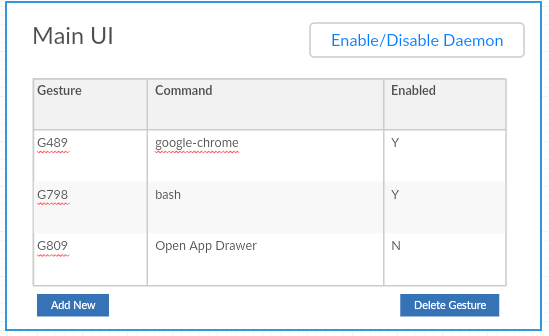
\includegraphics[scale=0.8]{mainui.png}
    \\
    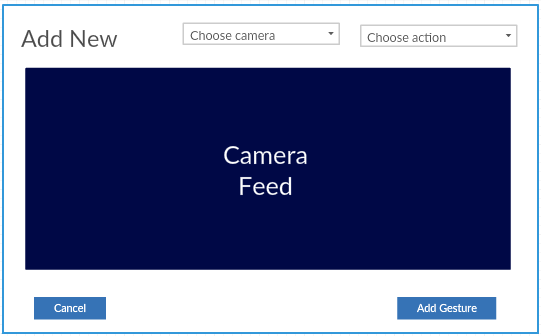
\includegraphics[scale=0.8]{addnewui.png}
\end{center}


\section{Hardware Interfaces}
The hardware required for the application is the webcam. The images are then handled by our application and the webcam too is managed by our deamon running in the background.

\section{Software Interfaces}
The daemon must interface with the camera driver and the operating system to be able to control the GUI based on input gestures.

\section{Communications Interfaces}
The application will need internet connection to send bug reports in case of a crash or malfunction. Bug reports will be sent in the form of HTTP requests to a remote webserver.

\chapter{Hardware and Software Requirements}
\section{Hardware Requirements}
\begin{itemize}
    \item A computer with at least 2GHz processor, 1GB RAM and USB ports.
    \item A USB camera.
\end{itemize}
\section{Software Requirements}
\begin{itemize}
    \item Linux operating system.
    \\
    \\The linux operating system was chosen due to the fact that it is easy to build software due to wide range of libraries and easy access to them and the compilers. Whereas in a OS like windows a special IDE like Visual Studio and proprietary libraries would be required to build software.
    \item C++ compliler eg:- gcc
    \\
    \\C++ is a general-purpose programming language. It has imperative, object-oriented and generic programming features, while also providing facilities for low-level memory manipulation.

    It was designed with a bias toward system programming and embedded, resource-constrained and large systems, with performance, efficiency and flexibility of use as its design highlights. C++ has also been found useful in many other contexts, with key strengths being software infrastructure and resource-constrained applications, including desktop applications, servers (e.g. e-commerce, Web search or SQL servers), and performance-critical applications (e.g. telephone switches or space probes). C++ is a compiled language, with implementations of it available on many platforms.
    \\
    \\Some of the interesting features of C++ are:
    \begin{itemize}
        \item \textbf{Object-oriented}: C++ is an object-oriented programming language. This means that the focus is on “objects” and manipulations around these objects. Information about how these manipulations work is abstracted out from the consumer of the object.
        \item \textbf{Rich library support}: Through C++ Standard Template Library (STL) many functions are available that help in quickly writing code. For instance, there are standard libraries for various containers like sets, maps, hash tables, etc.
        \item \textbf{Speed}: C++ is the preferred choice when latency is a critical metric. The compilation, as well as the execution time of a C++ program, is much faster than most other general purpose programming languages.
        \item \textbf{Compiled}: A C++ code has to be first compiled into low-level code and then executed, unlike interpreted programming languages where no compilation is needed.
        \item \textbf{Pointer Support}: C++ also supports pointers which are widely used in programming and are often not available in several programming languages.
    \end{itemize}
    \item OpenCV C++ library
    \\
    \\OpenCV (Open source computer vision) is a library of programming functions mainly aimed at real-time computer vision. OpenCV is written in C++ and its primary interface is in C++. All of the new developments and algorithms in OpenCV are now developed in the C++ interface. 
    \\
    \\OpenCV has a modular structure, which means that the package includes several shared or static libraries. The following modules are available:
    \begin{itemize}
        \item \textbf{Core functionality (core)} - a compact module defining basic data structures, including the dense multi-dimensional array Mat and basic functions used by all other modules.
        \item \textbf{Image Processing (imgproc)} - an image processing module that includes linear and non-linear image filtering, geometrical image transformations (resize, affine and perspective warping, generic table-based remapping), color space conversion, histograms, and so on.
        \item \textbf{Video Analysis (video)} - a video analysis module that includes motion estimation, background subtraction, and object tracking algorithms.
        \item \textbf{Camera Calibration and 3D Reconstruction (calib3d)} - basic multiple-view geometry algorithms, single and stereo camera calibration, object pose estimation, stereo correspondence algorithms, and elements of 3D reconstruction.
        \item \textbf{2D Features Framework (features2d)} - salient feature detectors, descriptors, and descriptor matchers.
        \item \textbf{Object Detection (objdetect)} - detection of objects and instances of the predefined classes (for example, faces, eyes, mugs, people, cars, and so on).
        \item \textbf{High-level GUI (highgui)} - an easy-to-use interface to simple UI capabilities.
        \item \textbf{Video I/O (videoio)} - an easy-to-use interface to video capturing and video codecs.
    \end{itemize}


    OpenCV has functions available for background subtraction. Several algorithms were introduced for this purpose. OpenCV has implemented three such algorithms which are very easy to use like BackgroundSubtractorMOG, BackgroundSubtractorMOG2 and BackgroundSubtractorGMG.
    
    OpenCV also has various feature extractors that can be used for detect the fingers of the user like CvFeatureEvaluator, CvFeatureParams, CvHaarEvaluator and CvHaarFeatureParams.
    \item GTK+ Library for C++
    \\
    \\GTK+, or the GIMP Toolkit, is a multi-platform toolkit for creating graphical user interfaces. Offering a complete set of widgets, GTK+ is suitable for projects ranging from small one-off tools to complete application suites.
    \\
    \\The GTK+ Library is needed to build an interactive GUI where users can configure the Gesture Control System. Functions to create windows and other GUI elements such as buttons, lists, pop-ups, drop-downs, frames to display video, etc are available in the library. The library also allows to bind functions to events in the GUI such as clicks, key-presses and so on.
    \\
    \\Features of GTK+:
    \begin{itemize}
        \item \textbf{Stability}: GTK+ has been developed for over a decade to be able to deliver the enticing features and superb performance that it brings to your application development. GTK+ is supported by a large community of developers and has core maintainers from companies such as Red Hat, Novell, Lanedo, Codethink, Endless Mobile and Intel.
        \item \textbf{Interfaces}: GTK+ has a comprehensive collection of core widgets and interfaces for use in your application.
        \item \textbf{Cross Platform}: Originally GTK+ was developed for the X Window System but it has grown over the years to include backend support for other well known windowing systems. Today you can use GTK+ on Windows, Mac OS X and Linux.
        \item \textbf{Accommodating}: GTK+ caters for a number features that today's developers are looking for in a toolkit including Native look and feel, Theme support, Thread safety and Object oriented approach.
        \item \textbf{Foundation}: GTK+ is built on top of GLib. GLib provides the fundamental algorithmic language constructs commonly duplicated in applications.
    \end{itemize}
\end{itemize}


\chapter{Functional Requirements}
\section{Start/Stop the Hand Gesture Daemon}
A toggle button that starts and stops the deamon which tracks hand gestures.
\begin{center}
    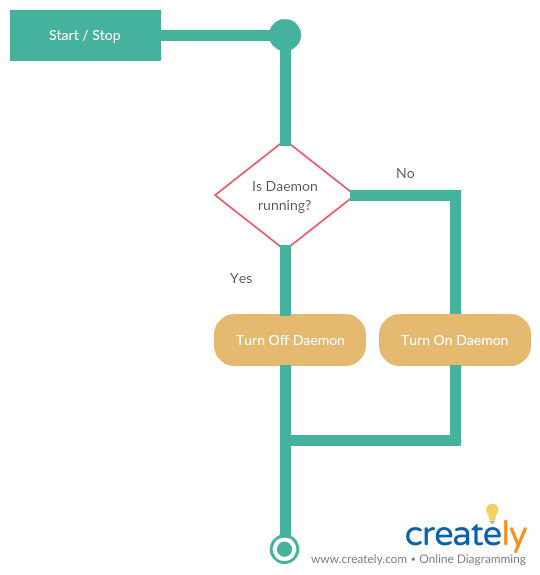
\includegraphics[scale=0.5]{start.png}
\end{center}
Input: Toggle button
\\Process: Will stop/start the daemon in the background
\\Output: The daemon shall be stopped/started.

\newpage
\section{Add new gestures}
The user should be able to add new gestures by recording the hand movement and mapping the GUI feature to the current Hand gesture.
\begin{center}
    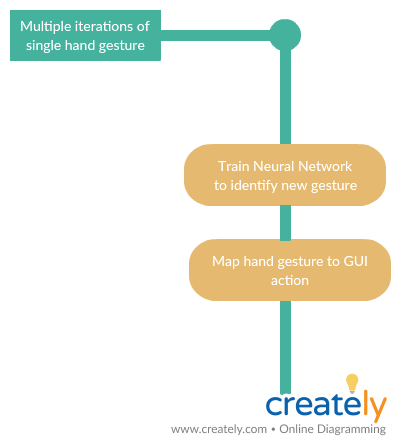
\includegraphics[scale=0.5]{add.png}
\end{center}
Input: Multiple Iterations of a gesture via Camera; Action to carry out
\\Process: The software will train the Neural Network to identify the new hand gesture and map the hand gesture to the Command given as input
\\Output: A new mapping from the hand gesture to the command will be added

\newpage
\section{Remove gestures}
The user can remove the existing gestures
\begin{center}
    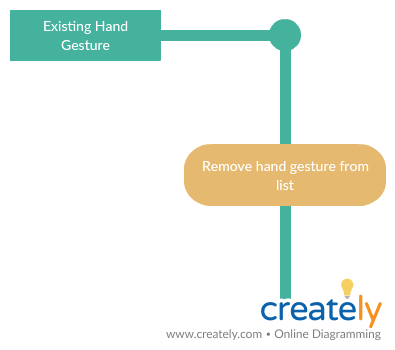
\includegraphics[scale=0.5]{remove.png}
\end{center}
Input: A hand gesture
\\Process: The software will remove the mapping of the input hand gesture from the list of hand gestures
\\Output: The hand gesture is removed
 
\newpage
\section{Modify Gestures}
\begin{center}
    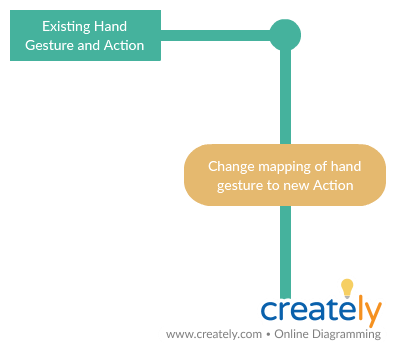
\includegraphics[scale=0.5]{modify.png}
\end{center}
Input: Existing hand gesture; Action to execute
\\Process: The software will change the mapping of the input hand gesture to the input Action
\\Output: The hand gesture is modified

\newpage
 \section{Choose webcam}
For systems with multiple webcams connected the user must be able to choose which webcam the application must use.
\begin{center}
    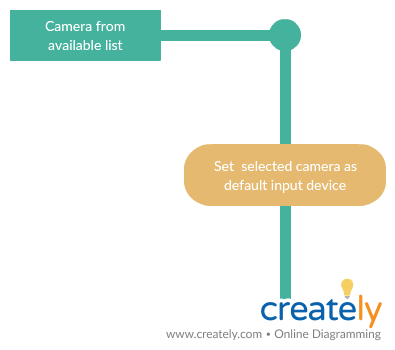
\includegraphics[scale=0.5]{camera.png}
\end{center}
Input: A camera detected by the daemon
\\Process: The software will set the selected camera as the default input for images
\\Output: The daemon will now watch for gestures through the selected camera when activated

\chapter{Other Nonfunctional Requirements}

\section{Performance Requirements}
The product must be fast enough to recognize and execute the hand gesture such that the action becomes fluid. The product must be responsive all the time and multiple hand gestures shown rapidly must be processed effectively.

\section{Safety Requirements}
No other application or user should access the camera feed.

\section{Security Requirements}
The camera feed must not be stored in the system. No one should be able to tap into the camera feed or be able to extract information from the camera.

\section{Software Quality Attributes}

Our product must be adaptable to all lighting conditions, poor webcams, and poor system capabilities. The product will be easy to maintain and review for other people. The  product will run on newer updates of the operating system without any glitches.



\chapter{Other Requirements}

The product can be reused by other developers to create and maintain their own products. The GUI of the application must work with all languages so that people from all backgrounds can work seamlessly. 



\begin{thebibliography}{999}
\addcontentsline{toc}{chapter}{References}

\bibitem{ } REAL TIME HAND GESTURE RECOGNITION
SYSTEM FOR DYNAMIC APPLICATIONS , Siddharth S. Rautaray , Anupam Agrawal, 2012

\end{thebibliography}

\end{document}